\documentclass[aspectratio=169,10pt]{beamer}

%\usepackage[utf8x]{inputenx}
\usepackage{hyperref}
\usepackage[spanish]{babel}

\usepackage{soul}

\usepackage[style=apa,backend=biber]{biblatex}
\addbibresource{bibliography.bib}
\renewcommand*{\citesetup}{%
	\footnotesize
	\biburlsetup
	\frenchspacing}

\usetheme{Marburg}
%\usecolortheme{beaver}

\title[Network Models]{Overview of Network Models}

\author[ggvy.cl]{George G. Vega Yon, Ph.D.}
\date{April 8th, 2022\\Network Science and Social Networks at the U (NETSNAU)}
\institute[UofU Epi]{Division of Epidemiology\\University of Utah}

\begin{document}

\frame{\maketitle\vfill\hfill  \href{https://ggvy.cl}{\texttt{ggvy.cl}}}

\begin{frame}
	\frametitle{Contents}
\tableofcontents\pause
\vfill\hfill%
You can download the slides from \href{https://ggv.cl/slides/netsnau0}{\color{blue}{\texttt{ggv.cl/slides/netsnau0}}}
\end{frame}

\begin{frame}
	\frametitle{The question}
	``I have data ABC and hypotheses XYZ...\pause \bigskip
	\hfill\begin{minipage}{.8\linewidth}
		\raggedleft
		\Large What \textbf{method} should I use to\\\textbf{address these questions}?''
	\end{minipage}
\end{frame}

\section{Modeling Networks}

\frame{\title{Contents}\tableofcontents[currentsection]}

\begin{frame}
	\frametitle{Modeling Networks}
	Today (in a non-comprehensive survey)
	\pause
	\begin{itemize}
		\item Classical statistical analysis assumes observations distribute \textit{independently} and \textit{identically} to each other\pause{} (generally).\pause
		\item Social, genes, and other entities are non-independent by definition.\pause
		\item Assuming independence can lead to trouble (as little as bias and even incorrect inferences.)\pause
		\item Educational programs and training are on the rise.
	\end{itemize}\pause
	\vfill\hfill Nonetheless...
	\end{frame}

\begin{frame}
	\frametitle{Modeling Networks (cont. 1)}
	\begin{itemize}
		\item We now have more data.\pause
		\item More computational power \parencite{Hofman2021,Lazer2020}.\pause
		\item And many communities, e.g., \href{INSNA}{} and \href{NetSCi}{}, accelerating the science.\pause
\end{itemize}

\vfill\hfill\large We can (and should) have a more systematic view of modeling networks and complex systems.

\end{frame}

\begin{frame}
	\frametitle{Modeling \st{Networks} Complexity (cont. 2)}
	\begin{figure}
		\centering
		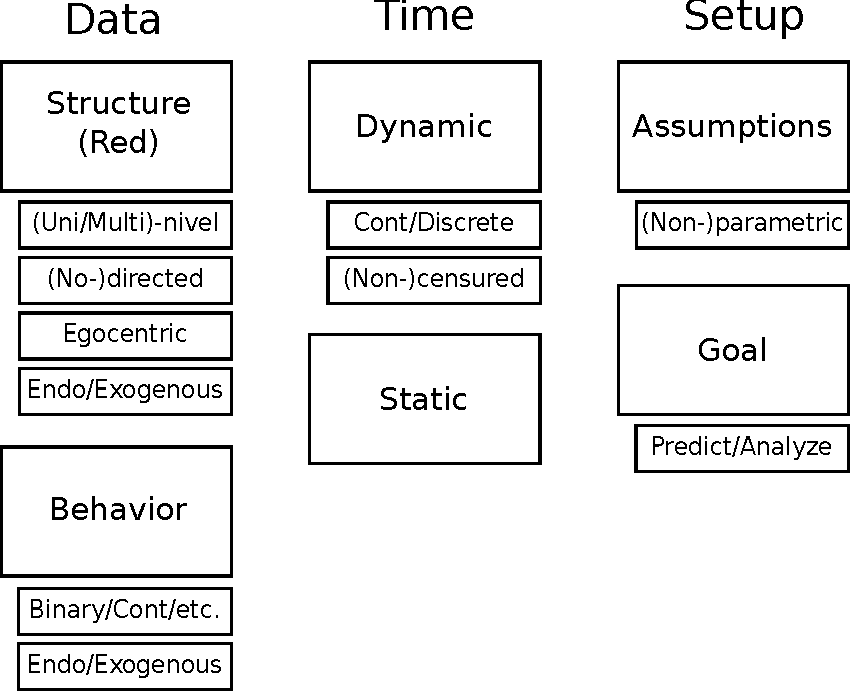
\includegraphics[width=.6\linewidth]{diagrama-en.pdf}
		\caption{Different dimensions of SNA (a view from the data.) All components interact with each other.}
	\end{figure}

\end{frame}

\section{Taxonomy of Methods}

\frame{\title{Contents}\tableofcontents[currentsection]}

\begin{frame}
	\frametitle{Taxonomy of Methods: A proposal}
	
	Two key dimensions, \textbf{structure} vs \textbf{behavior}, in particular\pause
	\begin{itemize}
		\item Structure: We just care about the network.\pause
		\item Behavior: Behavior given the existence of a network.\pause
		\item Structure x Behavior: We want to understand the co-evolution/distribution of network and behavior.
	\end{itemize}

\end{frame}

\subsection{Modeling Structure}

\begin{frame}
	\frametitle{Taxon: Structure}
\pause
	\textbf{Non-parametric}
	\begin{itemize}
		\item \textbf{Network Bootstrap} Standard errors and graph-level contrasts.
		\item \textbf{Network rewiring algorithms (e.g. CUG test)} \textit{Motifs} detection conditioning on observables (e.g., sequence or degree distribution)
		\item \textbf{Quadratic Assignment Procedure (QAP)} Label permutation for hypothesis testing.
	\end{itemize}\pause	
	
	\textbf{Parametric}

	\begin{itemize}
		\item \textbf{Exponential Random Graph Models (ERGMs)} Including all its flavors, like, TERGMs, BERGMs, ERGMitos, etc.
		\item \textbf{Relational Event Models (REMs) y Dynamic Actor Network Models (DyNAMs)} Sequence of interactions throughout time.
	\end{itemize}

Ref: \textcite{Snijders1999,Butts2008b,Krackhardt1988,Robins2007,VegaYon2021,Caimo2014,Butts2008,Stadtfeld2017}
	
\end{frame}

\subsection{Modeling Behavior}

\begin{frame}
	\frametitle{Taxon: Behavior}
\pause	
	\textbf{Non-parametric}
	\begin{itemize}
		\item \textbf{Permutation tests}: Simple or conditioned (ej. en \textit{in-degree})
	\end{itemize}
\pause
	\textbf{Parametric}
	\begin{itemize}
		\item \textbf{Spatial Autocorrelation}: Like Moran's I.
		\item \textbf{Spatial Autoregressive Models}: Like GLMs, but assuming that errors are jointly distributed in a graph-like fashion.
		\item \textbf{Lagged regressions} Entities' behavior is a function of previous exposure to peers.
	\end{itemize}

Ref: \textcite{Butts2008b,Moran1950,LeSage2008,Valente2019}

\end{frame}

\subsection{Modeling Structure x Behavior}

\begin{frame}
	\frametitle{Taxon: Structure x Behavior}
\pause
	\textbf{Non-parametric}
	\begin{itemize}
		\item \textbf{Agent-Based Models (ABM)} Simulation of Complex systems.
		\item \textbf{(idem)} used for parameter estimation through, e.g., likelihood-free MCMC and Approximate Bayesian Computation (ABC).
	\end{itemize}
\pause
	\textbf{Parametric}
	\begin{itemize}
		\item \textbf{Stochastic Actor Oriented Model (SAOM)} Continuous Markov process in which individuals' behavior and embeddedness interact throughout time.
		\item \textbf{Discrete Exponential-Family Models (DEFMs)} Individuals make multiple decisions on behavior and ties simultaneously (on development by yours truly...).
	\end{itemize}

Ref: \textcite{Tisue2004,Snijders2010intro,Csille2010,Marjoram2003}

\end{frame}

\section{More on Modeling Complexity}

\begin{frame}
\frametitle{More on Modeling Complexity}
    
Too many other methods/themes out there:

\begin{itemize}
    \item Modeling evolution using dynamic programming (likelihoods on directed graphs) (biology and computer science.) \parencite{Felsenstein1981}
    \item Identifying key entities in networks (centrality measures, structural holes, etc.) \parencite{Bringmann2019}
    % \item Contagion and diffusion (cascades, SIR models, etc.)
    \item Micro to macro behavior in Cellular Automatons. \parencite{Wolfram1983}
    \item Bayesian Networks (treating variables as nodes.) \parencite{Heckerman2008}
    \item Networks of Gene products. \parencite{Hecker2009}
    \item Stochastic block models (multi-group networks.) \parencite{Holland1983}
    \item Signed graphs (e.g., balance theory, i.e., the friend of my friend is my friend.) \parencite{Cisneros2021}
    % \item Multi-layered graphs.
    \item Survey and sampling methods for networks (e.g., snowball sampling.) \parencite{Goodman1961}
    \item Statistical mechanics of complex systems \parencite{Albert2002,barabasi2016network}
    \item ...
\end{itemize}

\end{frame}

% \section{Discussion}

% \begin{frame}
% 	\frametitle{Conclusiones}
% 	\pause
% 	\begin{itemize}
% 		\item \textbf{Asumir independencia} no siempre es factible/útil, es más, todo lo contrario.\pause
% 		\item El \textbf{desarrollo} tecnológico y metodológico nos han \textbf{democratizado el análisis de sistemas complejos}.\pause
% 		\item Es importante crear un \textbf{marco teórico} para \textbf{guiar la práctica} del ARS (SNA).\pause
% 		\item Una primera propuesta: $\{\mbox{Estructura},\mbox{Comportamiento}\}$\pause
% 		\item Más en \url{https://gvegayon.github.io/appliedsnar}
% 	\end{itemize}
% \end{frame}

\begin{frame}
	\centering
	\Huge Thank you! \normalsize 
\titlepage%
\vfill\hfill  \href{https://ggvy.cl}{\texttt{ggvy.cl}}
\end{frame}

\begin{frame}[allowframebreaks=1]
	\frametitle{References}
	\printbibliography
\end{frame}

\end{document}